% Created 2017-12-04 Mon 16:34
% Intended LaTeX compiler: pdflatex
\documentclass[11pt]{article}
\usepackage[utf8]{inputenc}
\usepackage[T1]{fontenc}
\usepackage{graphicx}
\usepackage{grffile}
\usepackage{longtable}
\usepackage{wrapfig}
\usepackage{rotating}
\usepackage[normalem]{ulem}
\usepackage{amsmath}
\usepackage{textcomp}
\usepackage{amssymb}
\usepackage{capt-of}
\usepackage{hyperref}
\usepackage{minted}
\usepackage{pdflscape}
\usepackage{rotating}
\usepackage[Bjornstrup]{fncychap}
\usepackage[dvipsnames]{xcolor}
\usepackage{minted}
\usepackage[french, english]{babel}
\date{}
\title{}
\hypersetup{
 pdfauthor={Willian Ver Valen Paiva},
 pdftitle={},
 pdfkeywords={},
 pdfsubject={},
 pdfcreator={Emacs 27.0.50 (Org mode 9.1.2)}, 
 pdflang={English}}
\begin{document}

\begin{titlepage}
\begin{center}

% Upper part of the page. The '~' is needed because only works if a paragraph has started.

\textsc{\LARGE}\\[1.5cm]

\textsc{\Large}\\[0.5cm]

% Title

\vspace{1cm}
\hrule
\vspace{1cm}


{\huge \bfseries Face alignment using deep learning}


\vspace{1cm}
\hrule
\vspace{1cm}


% Author and supervisor
\begin{minipage}{0.4\textwidth}
\emph{Author:} \\
Ver Valem Paiva \textsc{Willian}\\
\end{minipage}

\vfill

% Bottom of the page
{\large \today}

\end{center}
\end{titlepage}


\tableofcontents
\newpage


\section{Definition}
\label{sec:org6fa9d3d}

\subsection{introduction}
\label{sec:org5235ca7}

For a long time work in facial recognition has being done and one of the key
points of it is face alignment as it poses its own challenge.
And the main tool used for the job is OpenCV which is used with DLIB to
recognize Facial landmarks.

The automatic recognition of landmarks is essential to be able to classify
facial expressions, or face tracking, face animation, and even 3D face
modeling.

For example to classify facial expressions it is necessary to classify
Facial Action Units also known as FACS \cite{ekman1977facial}, which in turn
needs a proper face alignment.

The problem of face alignment is among the most popular in the field of
computer vision and today we have many different implementations to
automatically recognize facial landmarks on images.
The most known is the Active Appearance Model (AAM)
\cite{edwards1998face,matthews2004active}.

But today we also some good results using Deep learning to achieve the
results for example the work done by Adrian Bulat on recognizing 3D facial
landmarks \cite{bulat2017far} that shows remarkable results and is implemented
in \emph{Torch} a framework for \textbf{LUA}. 

As the DLIB model has difficulty on recognizing points on faces by the side
view, this project focus on this problem and does its best to tackle this
problem.

\subsection{Problem Statement}
\label{sec:orgd6a46cc}

The problem in question take a image as input (the format and details will be
discussed on the dataset section), and by using a regression model to
calculate the position of the face landmarks on the given image.

For that the models used to tackle this problem will output 152 numbers, where
each number ranges from 0 to 1 and represents the X and Y of each of the 76
landmarks. 

The expected result is a model capable precisely recognize the set of
landmarks.


\subsection{Metrics}
\label{sec:orgfa6d0b9}

The results of this project was avaliated using the Mean Squared Error (MSE) 
this metrics was chosen as it is standard function for regression problems
and it fits well problem in question. 

\section{Analysis}
\label{sec:orga8c8fbe}

\subsection{Dataset}
\label{sec:org2d8f80a}
In this study the MUCT Face Database \cite{Milborrow10} was used
this dataset consists of pictures (resolution 480x640) taken from 276 subjects
using 5 cameras in different angles and light conditions (total of 3755
images) like the image below: 

\begin{figure}[htbp]
\centering
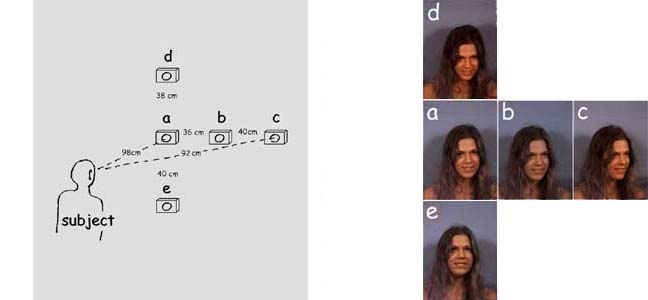
\includegraphics[width=.9\linewidth]{./images/muct-views-lores.jpg}
\caption{There is no images on the left but they can be reproduced by mirroring the right side}
\end{figure}

Each picture is manually coded with 76 facial landmark like:
\begin{center}
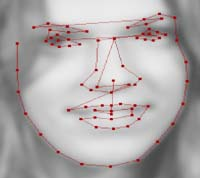
\includegraphics[width=.9\linewidth]{./images/landmarks.jpg}
\end{center}


The landmarks are saved in to 4 different file formats

\begin{itemize}
\item muct76.shape       shape file \cite{milborrow2009active}
\item muct76.rda         R data file (www.r-project.org/
\item muct76.csv         comma separated values
\item muct76-opencv.csv  comma separated values in OpenCV coords (0,0 at top left).
\end{itemize}


the coordinate system in these files is the one used by Stasm (i.e. the
origin 0,0 is the center of the image, x increases as you move right, y
increases as you move up).  The exception is muct76-opencv.csv, where the
format is the "OpenCV format" (i.e. the origin 0,0 is at the top left, x
increases as you move left, y increases as you move down). 

Unavailable points are marked with coordinates 0,0 (regardless of the
coordinate system mentioned above).  "Unavailable points" are points
that are obscured by other facial features.  (This refers to landmarks
behind the nose or side of the face -- the position of such landmarks
cannot easily be estimated by human landmarkers -- in contrast, the
position of landmarks behind hair or glasses was estimated by the
landmarkers).  

So any points with the coordinates 0,0 should be ignored.  Unavailable
points appear only in camera views b and c.  

the subjects 247 and 248 are identical twins.

The data set is available via \href{https://github.com/StephenMilborrow/muct}{github} or it is also a submodule on this
project and by recursively initializing or cloning the data can be found in 
folder project/dataset that is the recommended way as the scripts depend on
this folder 


\subsection{Split the training and testing sets}
\label{sec:org5af3151}

As this dataset is composed by multiple images of the same subject the
division of sets for training and testing could not be done at a random way
as an special attention is needed to not have the same subject on the train
and testing set.

And after analyzing it was divided by taken the first 82 subjects for the
testing set (249 images per camera total of 1245 around 30\%)

The function "decompress\(_{\text{dataset}}\)" on the \emph{DataGen.py} takes care of
decompressing the data and splitting the training and testing set. 

\subsection{Data Analyses}
\label{sec:org1cfc347}

lets start by looking at one image from the database those images are on the
format of 640x480. 
\begin{center}
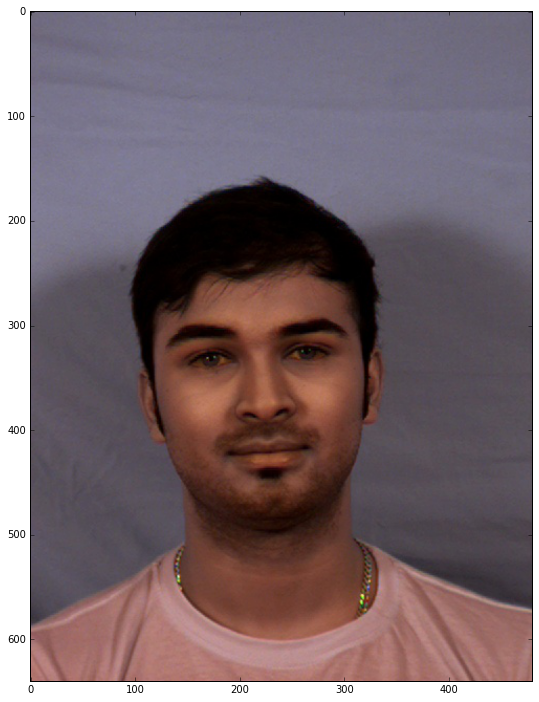
\includegraphics[width=.9\linewidth]{./images/example1.png}
\end{center}

And lets plot the points on one image to have an insight: 

\begin{center}
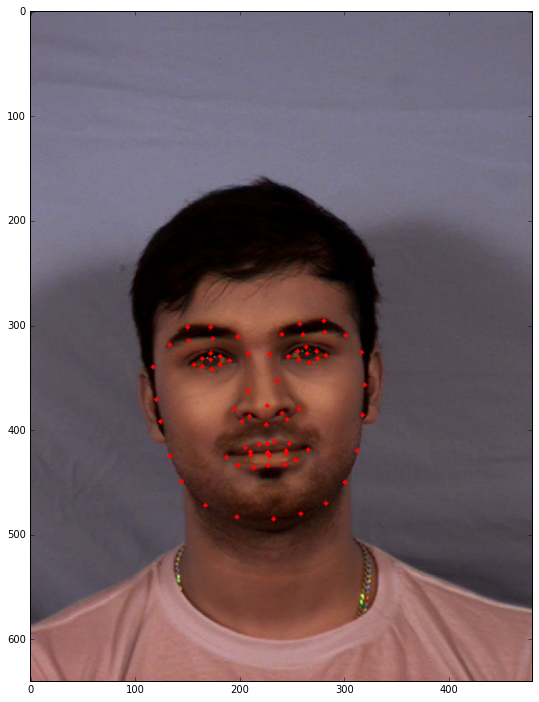
\includegraphics[width=.9\linewidth]{./images/example2.png}
\end{center}

As is possible to see those images are large and have big regions with
useless information like the background.

To improve that lets use DLIB's face recognition to find the face area and
crop it, for that we can use the function "crop$\backslash$\(_{\text{image}}\)" from the \emph{DataGen.py} 
this function takes the image and the size to crop we pass just one integer
for the size as it crops the image in a square, and returns the cropped image
and the bound box used to crop the image. 

\begin{figure}[htbp]
\centering
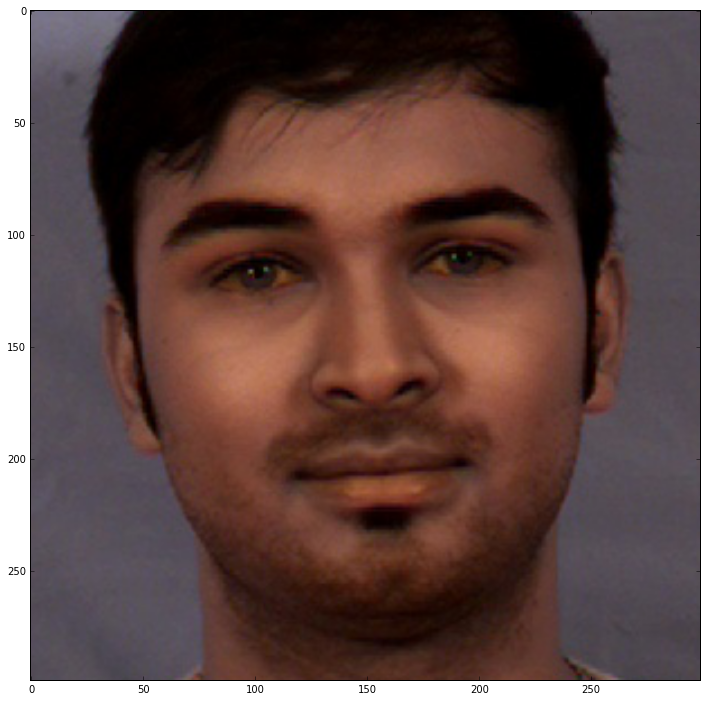
\includegraphics[width=.9\linewidth]{./images/example3.png}
\caption{image cropped with the size of 299 x 299.}
\end{figure}

But as the image have being cropped we also have to move the landmark points
to match the new image, for that we can use the function "replace$\backslash$\(_{\text{landmarks}}\)"
which takes the bound box and the actual landmarks and return the new
landmarks

\begin{center}
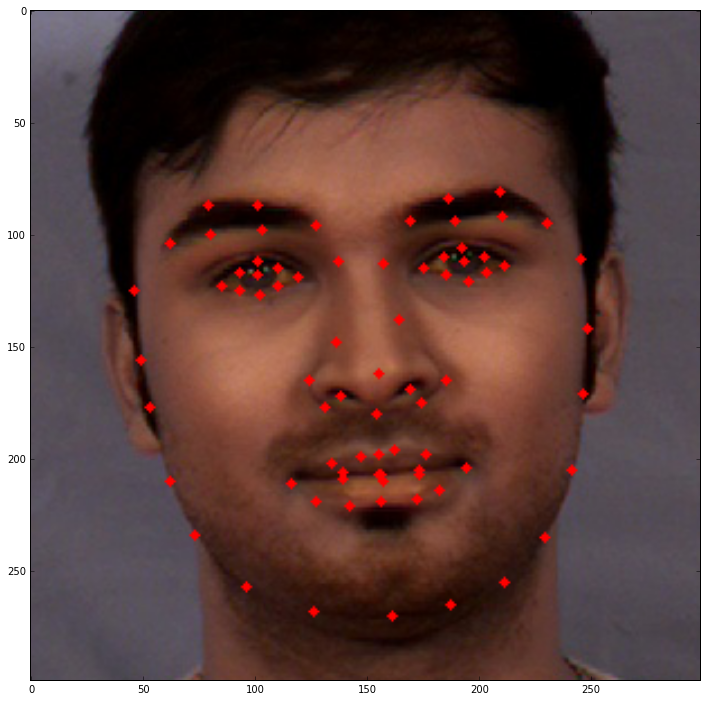
\includegraphics[width=.9\linewidth]{./images/example4.png}
\end{center}

the process of cropping the image brings 2 advantages to the project:
\begin{itemize}
\item less resources needed to train model
\item it makes possible to use images with more than one face in the future
\end{itemize}

\subsection{Data Augmentation}
\label{sec:orgc7d9234}

As explained before there is no cameras on the left but we can mirror the
right images, starting from that we will implement a some data augmentation 
like flipping every image horizontally and vertically.

To achieve that we can use the function "flip$\backslash$\(_{\text{image}}\)" also from \emph{DataGen.py}
it takes the image, the landmarks, the direction to flip, width and height.
and returns the new image and landmarks.
lets see the result:

\begin{center}
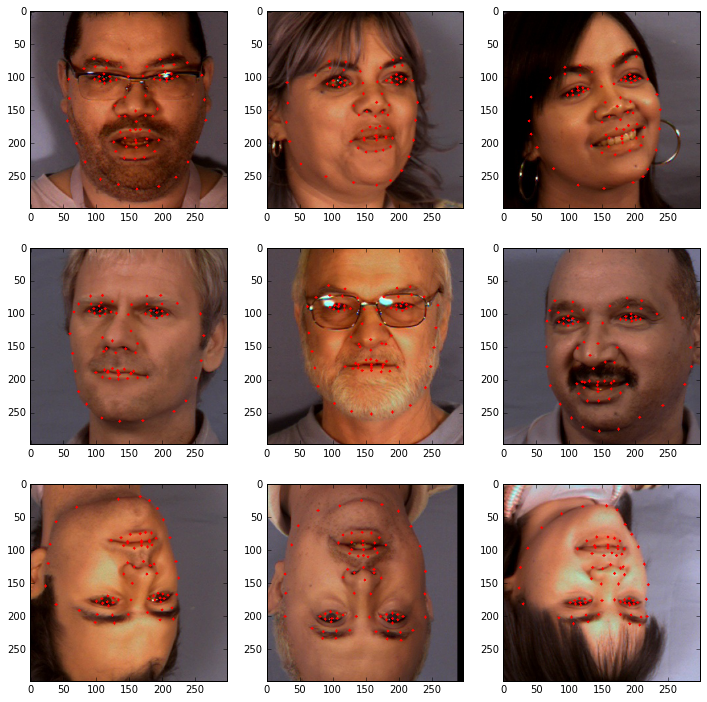
\includegraphics[width=.9\linewidth]{./images/example5.png}
\end{center}

By applying this to all images we finish with a total of 3723 testing images
and 7497 training images  

\subsection{Algorithms and Techniques}
\label{sec:org3a05739}

To tackle this problem 2 possibilities was taken in consideration:

\begin{enumerate}
\item The use of a fully convolutional network (FCN) and map the points by
returning the pixel of a landmarks
\item The use of a convolutional neural network (CNN) with a regression output
returning the coordinates of the landmarks
\end{enumerate}

While the 2 approaches are valid this project focused on the second one as
the first would require more experience and knowledge to do it.

The project is composed of 2 parts:
\begin{enumerate}
\item The CNN layer.
\item The regression output.
\end{enumerate}

All the models have 1 thing in common the \textbf{output} all the models have a
152 neurons dense layer using linear activation, used to predict the
coordinate of the landmarks on the image.
In the other hand the CNN part of every model is different, here the approach
was to develop a CNN capable to pass a precise information about the shape in
the image to the output layer so we could have a precise landmark on the
image. 


\subsection{Benchmark}
\label{sec:orgbe13fba}

To bench mark this project a model using a CNN created from scratch was used 
and the model and the results of this model can be seen at the \ref{sec:org046c0e7} \textbf{CNN from scratch} in the \ref{sec:org01aec23} \textbf{Implementation} section of
this report.  


\section{Methodology}
\label{sec:orgf42334f}

\subsection{Data Preprocessing}
\label{sec:org40651da}

Many steps of preprocessing have being taken and have being discussed on the
\ref{sec:org2d8f80a} section being then:
\begin{itemize}
\item Split of the data discussed at the \ref{sec:org5af3151}
\textbf{Split the training and testing sets} section
\item Image cropping detailed at the \ref{sec:org1cfc347} \textbf{Data Analyses} section
\item Data Augmentation described on the \ref{sec:orgc7d9234} \textbf{Data Augmentation} section
\item 
\end{itemize}
\subsection{Implementation}
\label{sec:org01aec23}

For this project many different approaches have being taken and it will be
presented here the best outcome of each "kind" of approaches like:

\begin{itemize}
\item A CNN created from scratch
\item Inception transfer learning
\item ResNet50 transfer learning
\end{itemize}

All the models have being trained in a cloud server for performance wise and
saved to later study.

The metrics used to observe the performance of every model was the mean square
error (MSE)

The models code can be found on the file \emph{Models.py}.

The models use a \emph{"npz"} file that can be generated via by using the function :
\begin{verbatim}
DataGen.save_dataset(DataGen.create_dataset(size, True, True), "outputName")
\end{verbatim}

And for the inception transfer learning it uses a bottleneck file that can be
generated with the function:

\begin{verbatim}
DataGen.inception_bottleneck(<npz file>, "outputName")
\end{verbatim}

every model was implemented using early stopping, TensorBoard and saves the
best loss weights on a \emph{hdf5} file   


\pagebreak

\subsubsection{CNN from scratch}
\label{sec:org046c0e7}

This CNN started with a model based on the AlexNet \cite{krizhevsky2012imagenet} 
\begin{center}
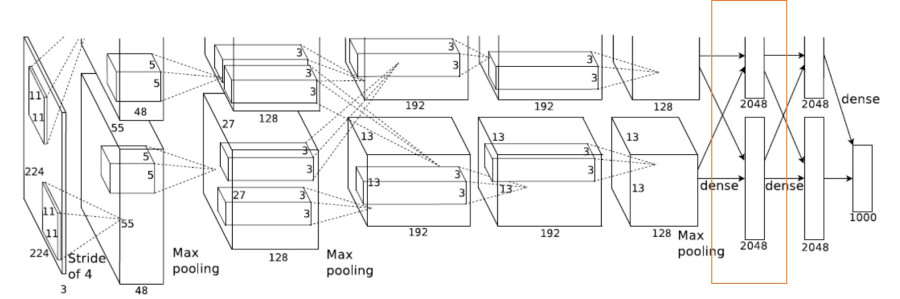
\includegraphics[width=.9\linewidth]{./images/alexnet6.jpg}
\end{center}
But we finished with a model as illustrated below:
\begin{figure}[htbp]
\centering
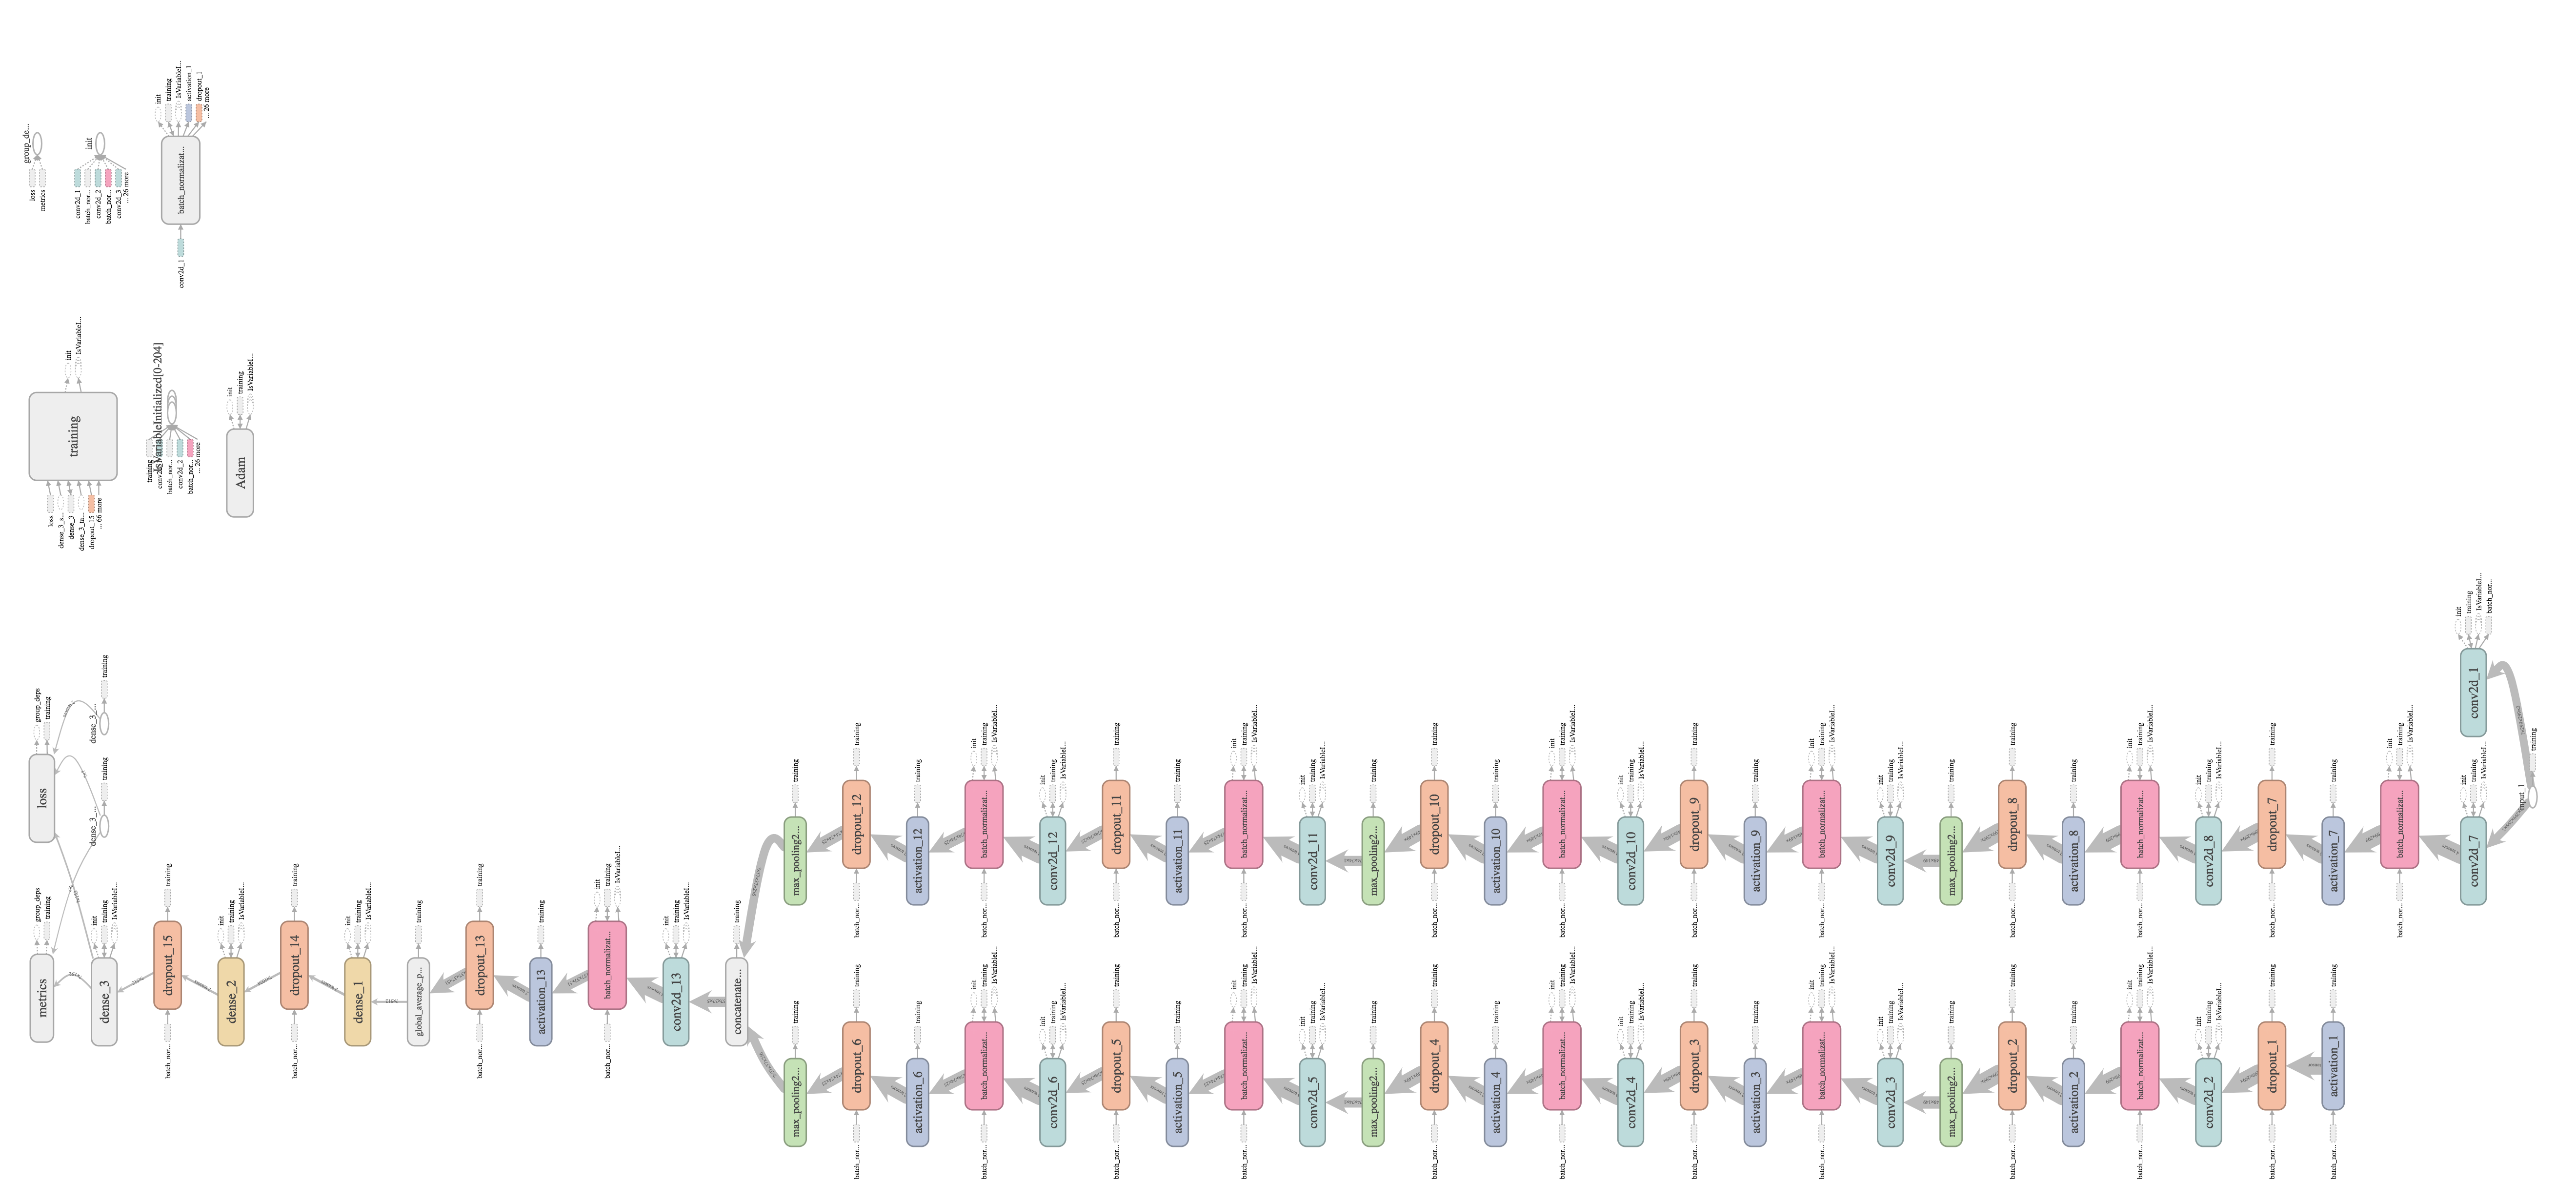
\includegraphics[width=.9\linewidth]{./images/mymodel.png}
\caption{the full size image can be found on the report/images/mymodel.png.}
\end{figure}

here is the learning curve from this model
\begin{center}
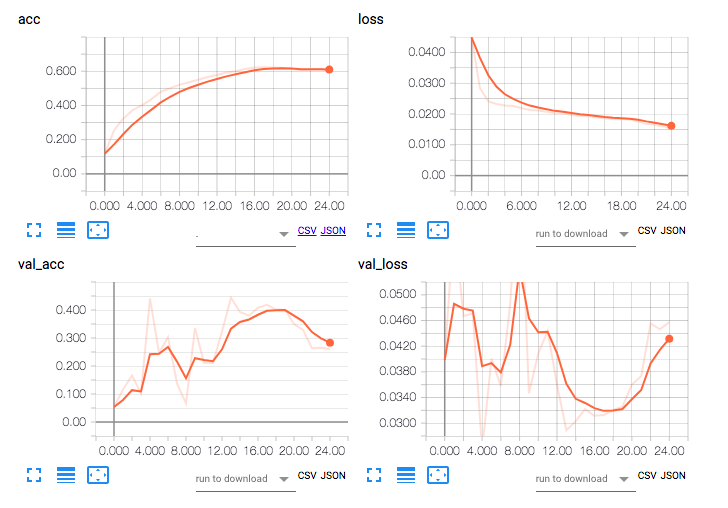
\includegraphics[width=.9\linewidth]{./images/mymodelLoss.png}
\end{center}

as we can see the learning curve for the training set was improving steadily
but for the testing set it starts to get worst  around the epoch 16 and the
early stopping is triggered at epoch 24 as it has no improvement.

by taking the weights of the best loss and doing an inference on a set of
training images we get the following result: 

\begin{center}
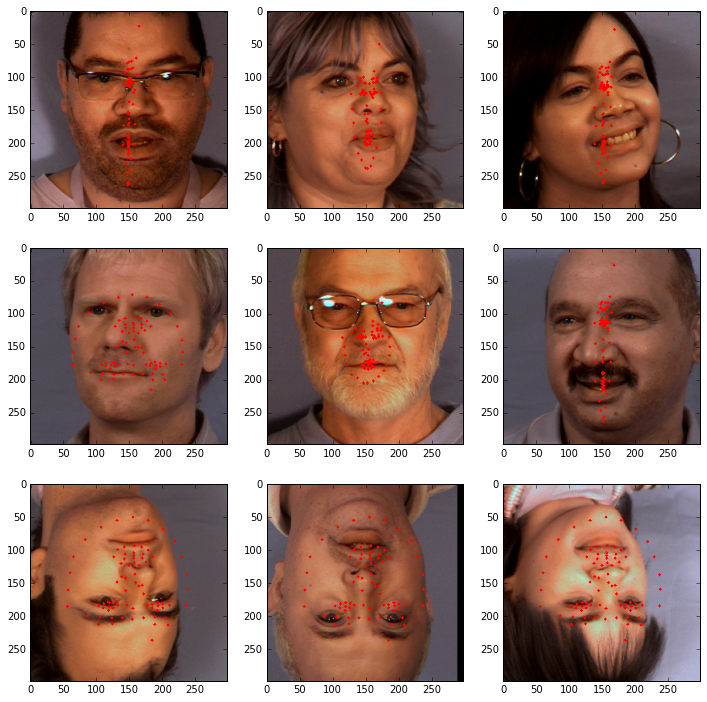
\includegraphics[width=.9\linewidth]{./images/mymodelTest.png}
\end{center}

It is noticible that the result is not satisfactory but it has plenty of room
for improvement. but at this point of the project it started to get expensive
to keep using the cloud machine to train and there was yet some other methods
to try out.  

\subsubsection{Inception transfer learning}
\label{sec:org04d8222}

\begin{enumerate}
\item bottleneck
\label{sec:org25e51c5}

The next step was to use transfer learning, by using the inceptionV3
\cite{szegedy2016rethinking}, the first approach as to create bottleneck files
from the inception and train a model with those outputs.

As the previous model many models have being made and here is the best result 
found by using this method was the following:

\begin{figure}[htbp]
\centering
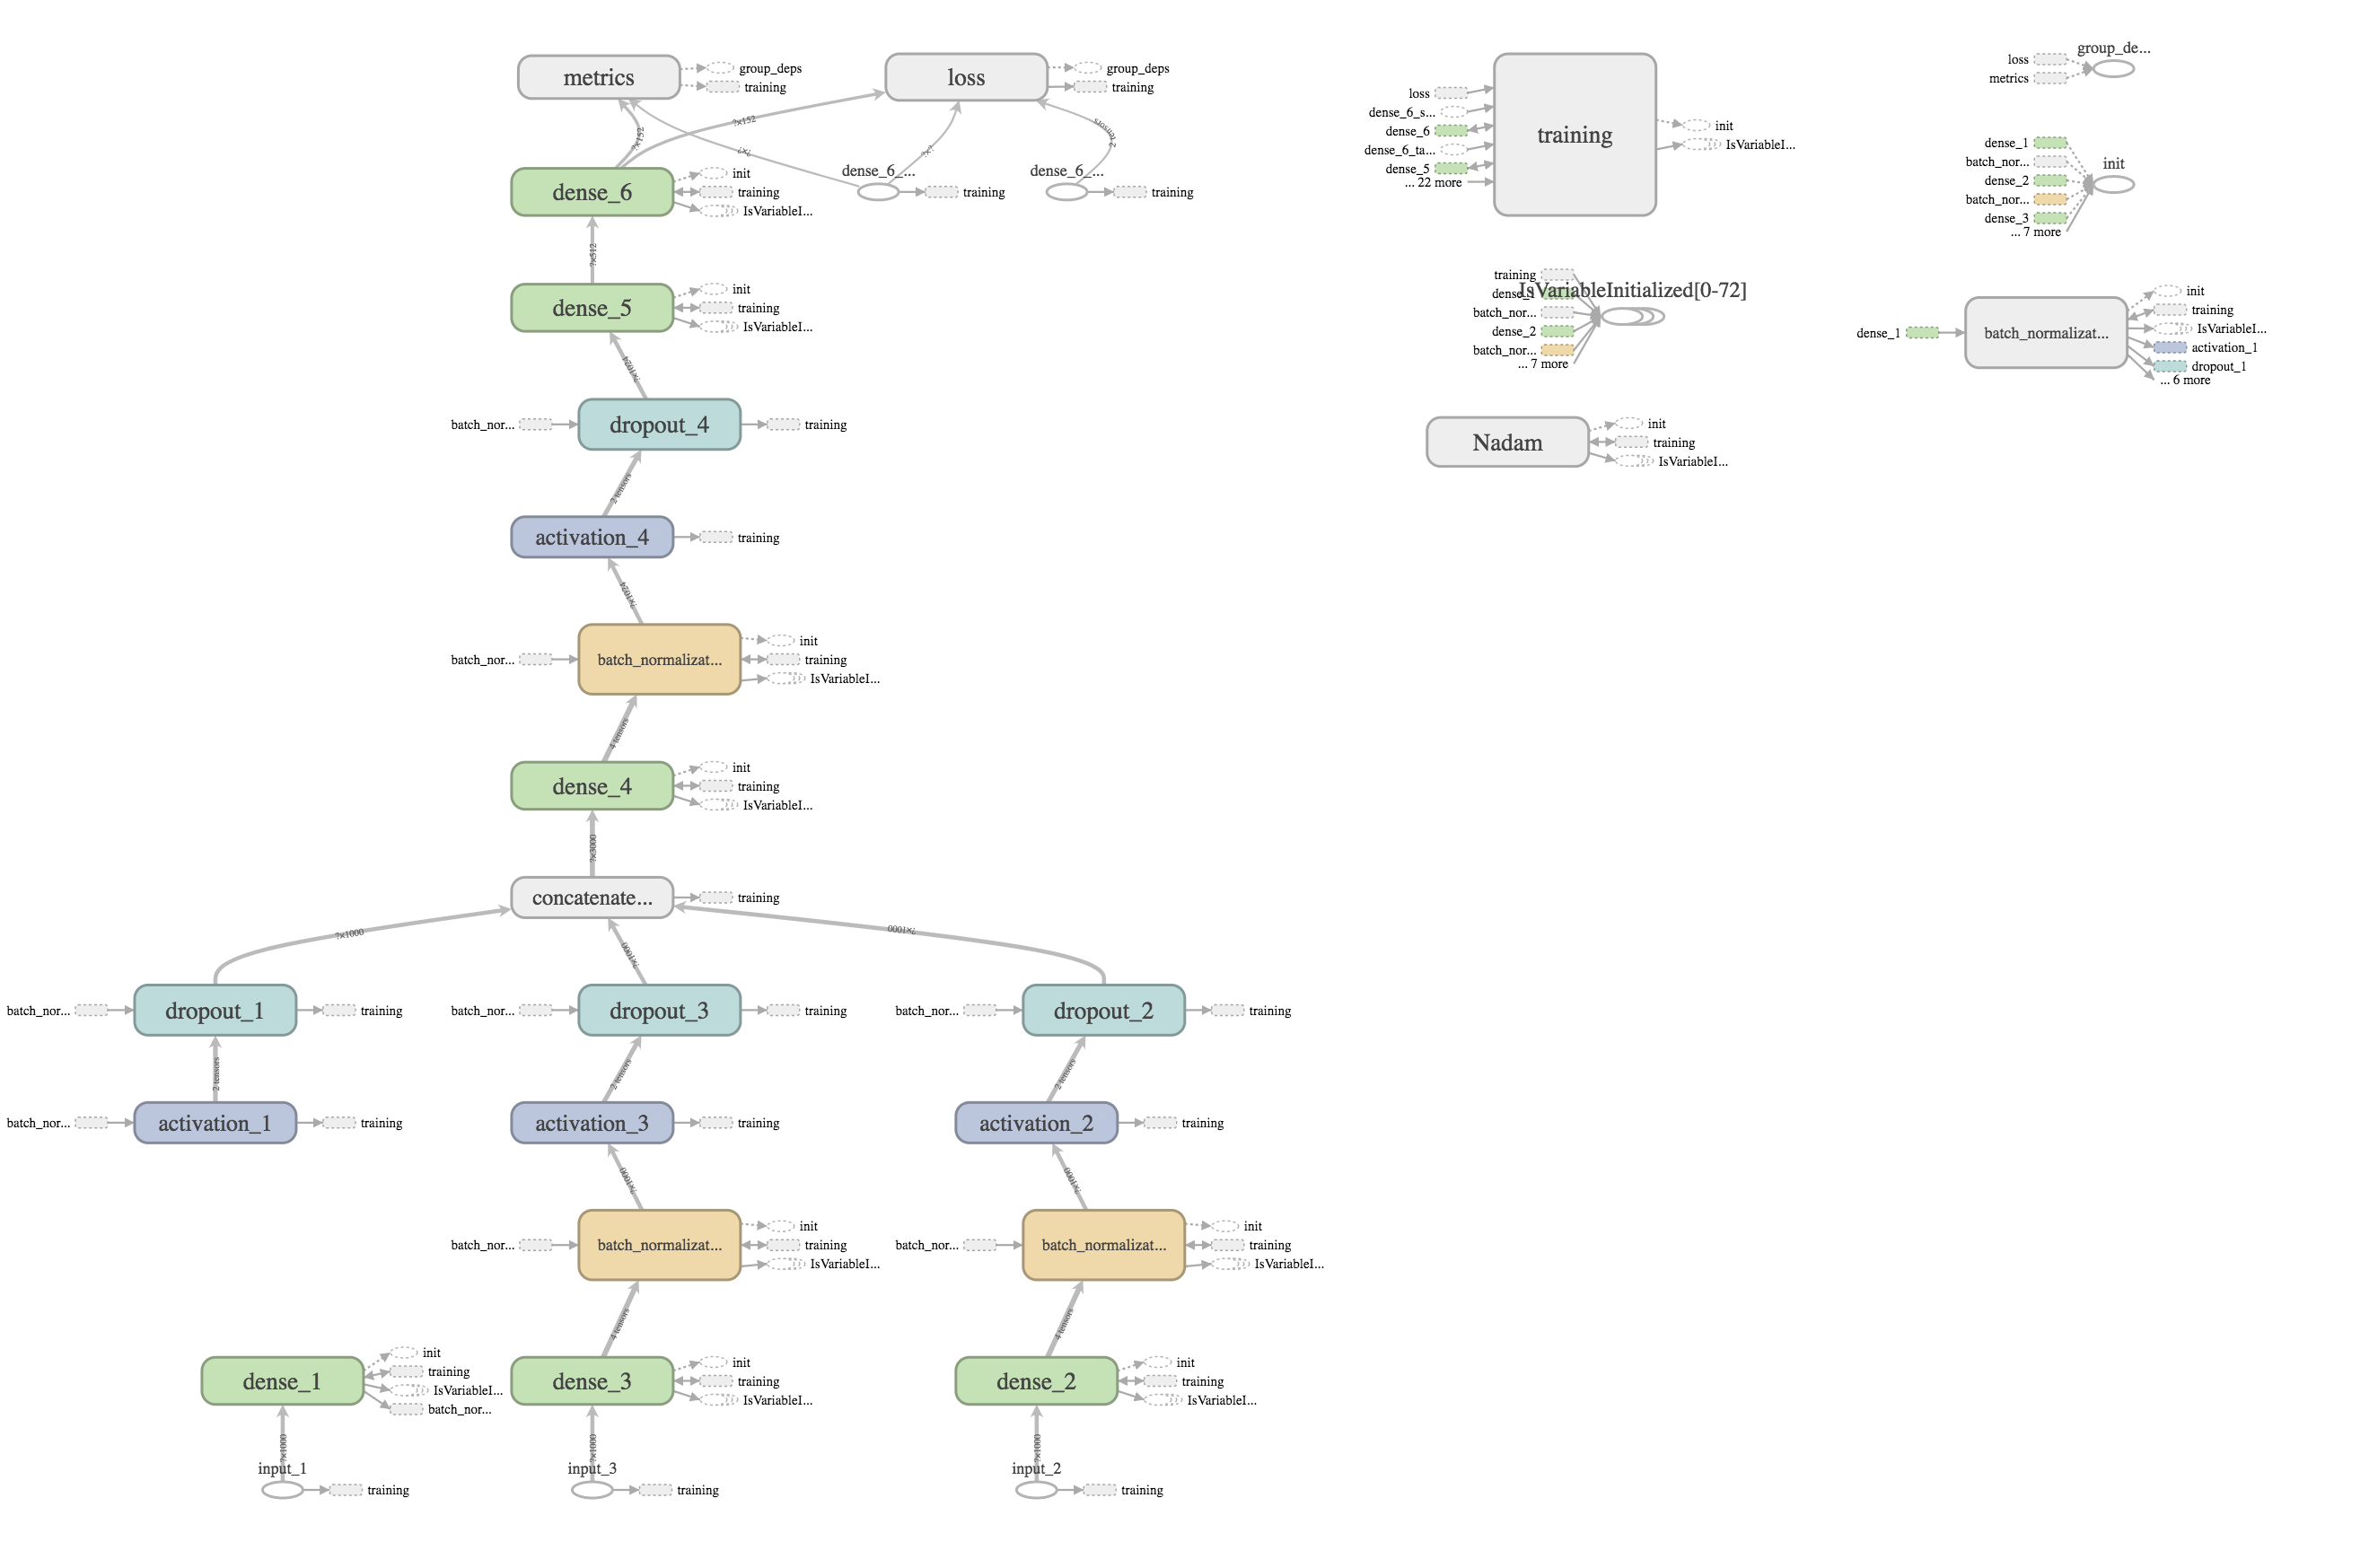
\includegraphics[width=.9\linewidth]{./images/btn.png}
\caption{the full size image can be found on the report/images/btn.png.}
\end{figure}

In this model we took a different approach as just using the output of
Inception wasn't given good results 3 different inputs was used the squared
and the \emph{sine} of the inception output was also used in conjunction to the
normal output 

\begin{center}
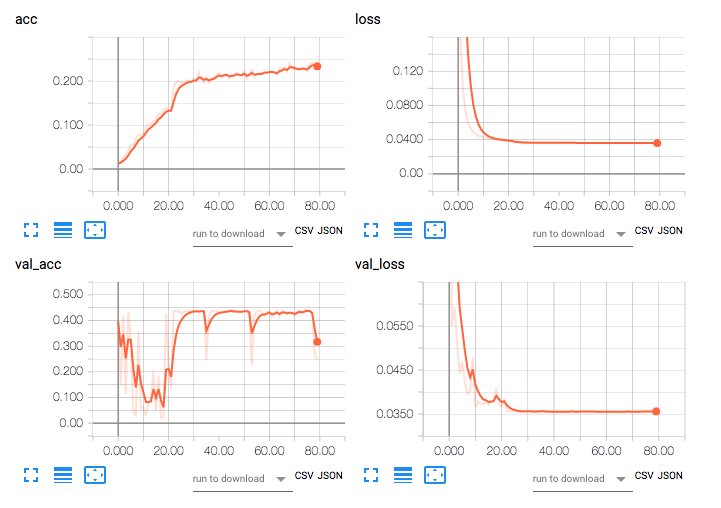
\includegraphics[width=.9\linewidth]{./images/btnLoss.png}
\end{center} 

The training of this model took 80 epochs before the early stopping was
triggered while the learning curve on the test set is better them the previous
model the loss is slightly bigger them the previous model:

\begin{center}
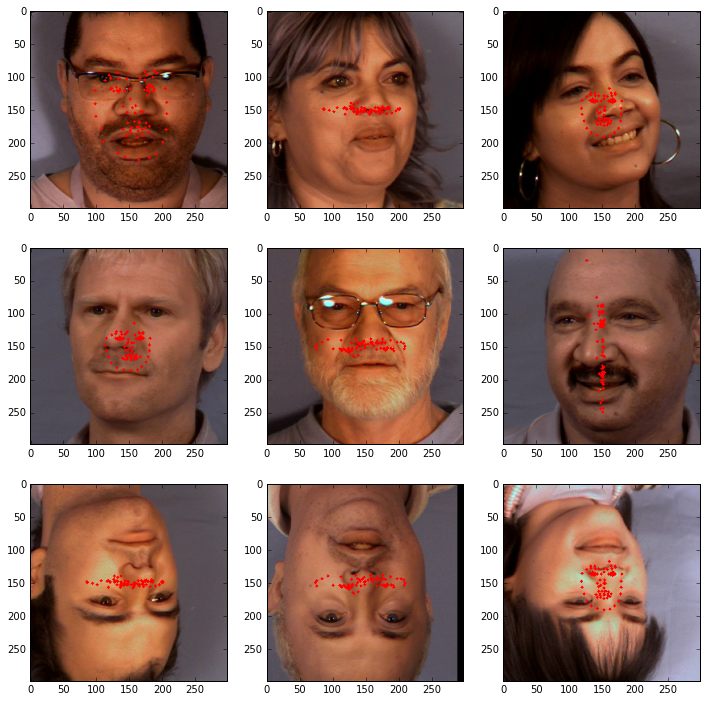
\includegraphics[width=.9\linewidth]{./images/btnResult.png}
\end{center}

And the results are far from good, worst then the previous model. 

\pagebreak


\item Retrain
\label{sec:orgecb06e1}

The next step here is to keep using the transfer learning from inception but
give a bit of more room for improvement by training respectively the 2 last
convolutional blocks of the inception and the 4 last ones:

\begin{figure}[htbp]
\centering
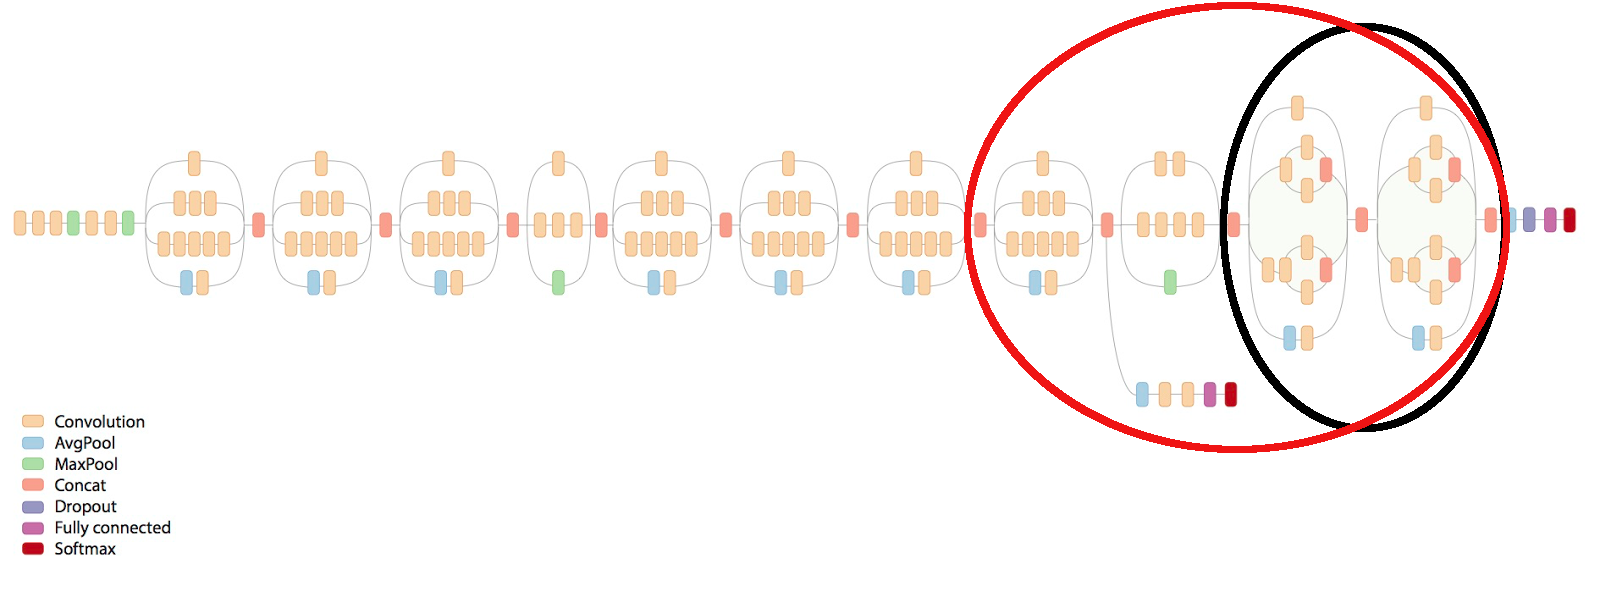
\includegraphics[width=.9\linewidth]{./images/incep.png}
\caption{4 block(red) 2 block(black).}
\end{figure}


\pagebreak

\begin{enumerate}
\item \textbf{2 blocks results}
\label{sec:org395fcaa}

\centerline{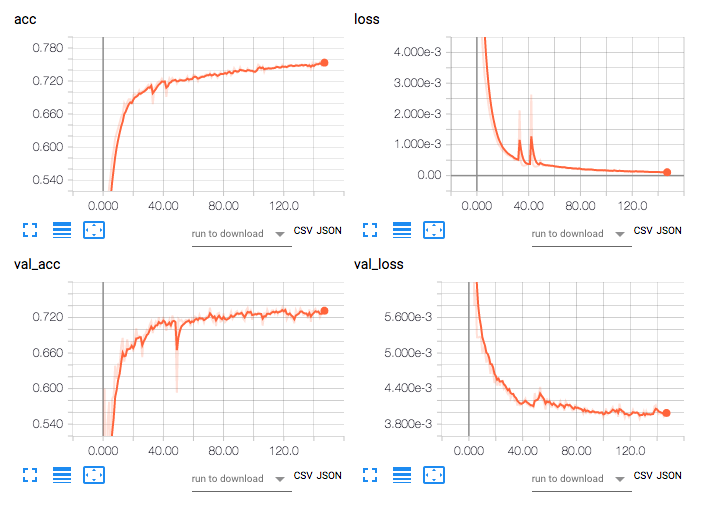
\includegraphics[height=9cm]{./images/incep249Loss.png}}
\centerline{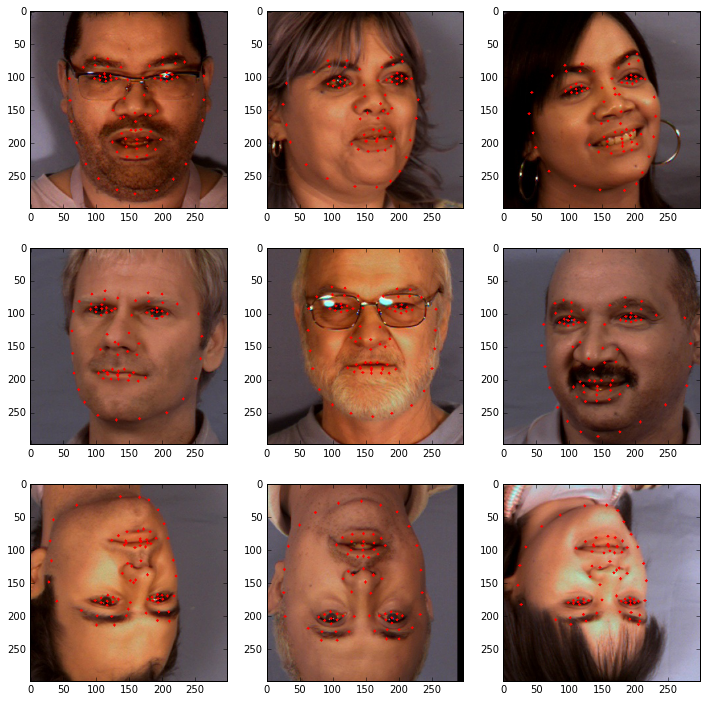
\includegraphics[height=9cm]{./images/incep249res.png}}

\pagebreak

\item \textbf{4 blocks results}
\label{sec:org6e232b6}

\centerline{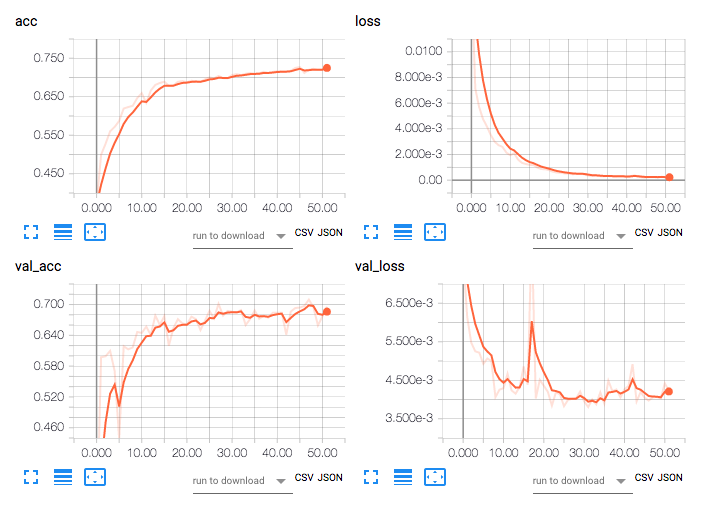
\includegraphics[height=9cm]{./images/incep197Loss.png}}
\centerline{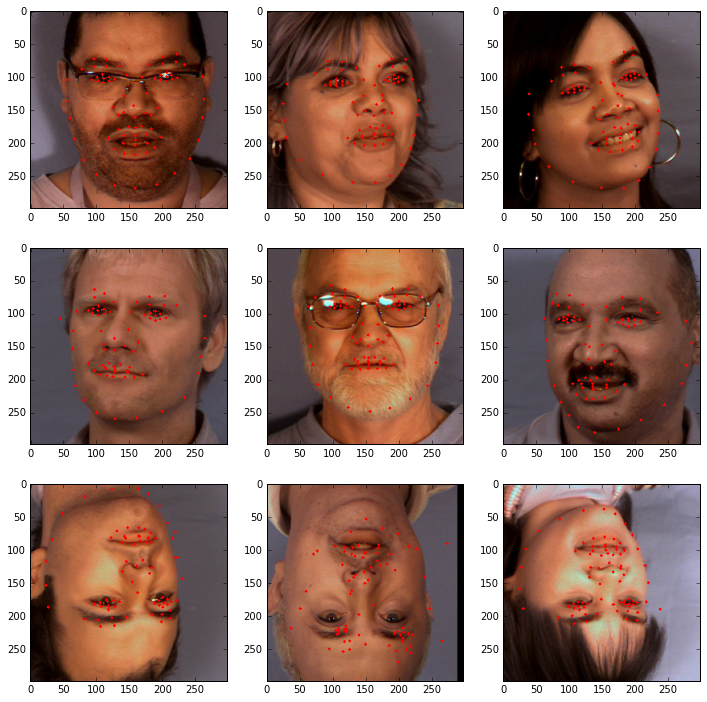
\includegraphics[height=9cm]{./images/incep197res.png}}


\pagebreak
as we can see it really improved the results by using the 2 first blocks after a
120 epochs we have a steady learning curve and we get a nice prediction on the
testing images, but once we increase the number of training layers by using
the first 4 block, the early stopping triggers 70 epochs before and while
the results look good, however, it is worst then the model with 2 blocks.
\end{enumerate}
\end{enumerate}


\subsubsection{ResNet50 transfer learning}
\label{sec:org12be8db}
Here the same approach that as used with Inception is used with the ResNet50 \cite{he2016deep}  
model, but as the ResNet50 uses images with format 224x224 and we have images
with 299x299, while we could crop the images it is not a good solution as it
was cutting out landmarks from some images. So the idea here is use the
ResNet50 with different input. 

2 models was trained here one that don't train any layer from ResNet50 and
another that trains 2 convolutional blocks like:

\begin{center}
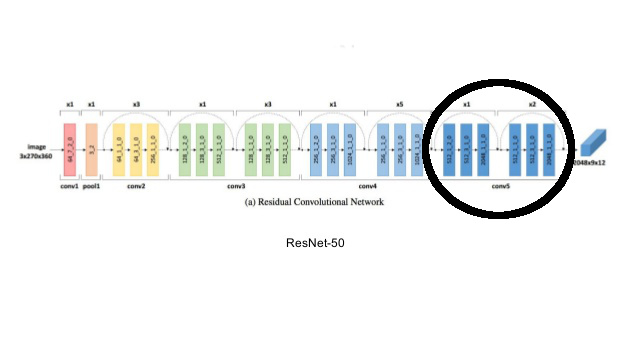
\includegraphics[width=.9\linewidth]{./images/resnet50.jpg}
\end{center}


\pagebreak

\begin{enumerate}
\item \textbf{0 blocks results}
\label{sec:org7f6063b}

\centerline{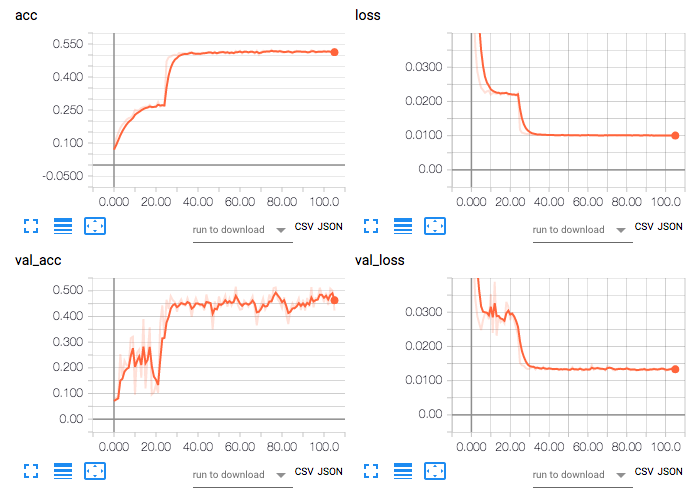
\includegraphics[height=9cm]{./images/resnet0loss.png}}
\centerline{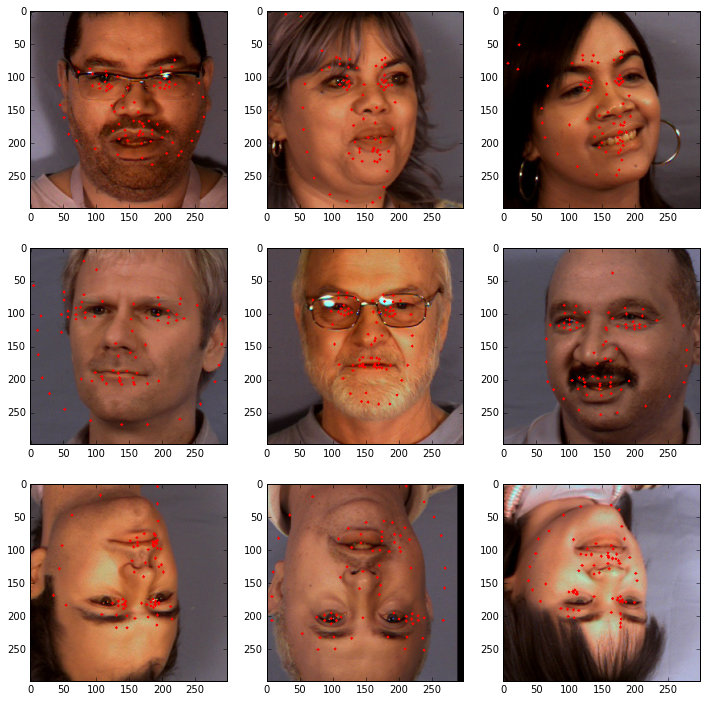
\includegraphics[height=9cm]{./images/resnet0res.png}}


\pagebreak
\item \textbf{2 blocks results}
\label{sec:orge5004e1}

\centerline{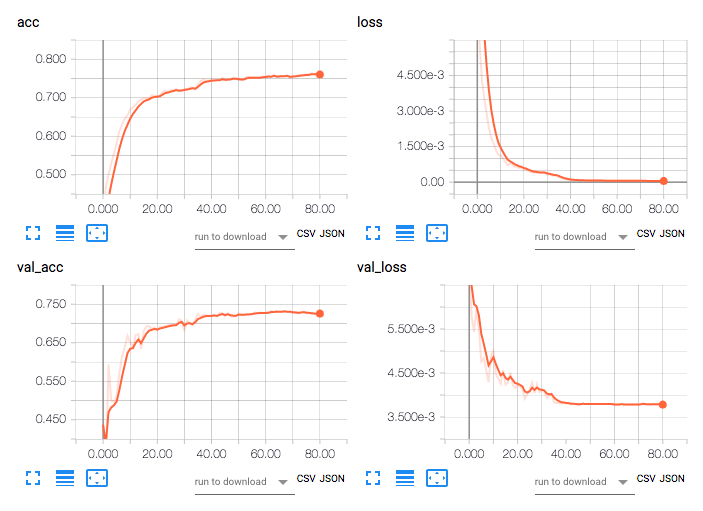
\includegraphics[height=9cm]{./images/resnet2loss.png}}
\centerline{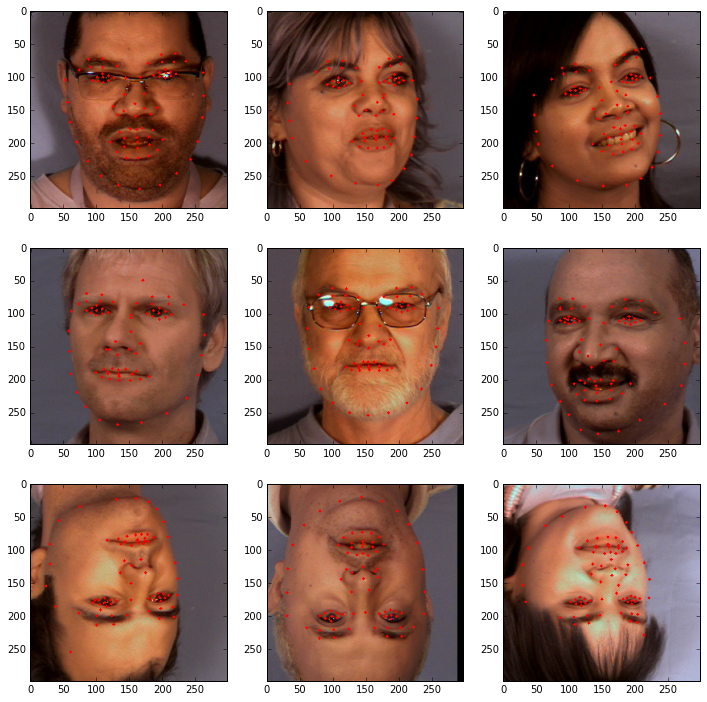
\includegraphics[height=9cm]{./images/resnet2res.png}}

\pagebreak
as it is noticible using just the output of ResNet50 did give better results
them the inception but yet it wasn't satisfactory in the other hand when
retraining 2 block it showed a really promising result
\end{enumerate}


\subsection{Refinement}
\label{sec:orgb8026d3}
while the results presented here are the best ones for each of the models 
many trials have been done the first tuning was working with the learning
and the optmizers and here is what was what was used:
\begin{enumerate}
\item SGD
\label{sec:org02772c1}
all results were poor with this optimizer

\item RMSprop
\label{sec:orgf1e329a}
that was the second optimizer tried it was a bit trick as the results were
showing all the points accumulating near of the center of the image like:

\begin{center}
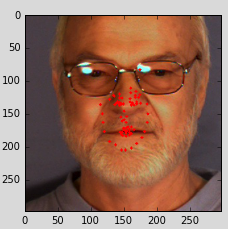
\includegraphics[width=.9\linewidth]{./images/RMSprop.png}
\end{center}

the approach to fix it was to increase the learning rate to 0.1 and use a
learning rate decay until 0.0001 while that give better results, further
analyses showed that wasn't the best approach

\item Adam
\label{sec:org618d911}
this is the optimizer used on every model with exception of the benchmark
model and while the reduction of a learning rate showed improvement on some
other tests it was taking too long to train and exhausting the resources
for this project and we sticked with the Keras default learning rate

\item Nadam
\label{sec:org3d5913c}
This optimizer as used for the benchmark model and showed good results (no
tuning was made).
\end{enumerate}



\section{Results}
\label{sec:org206d1d0}

\subsection{Model evaluation and Validation}
\label{sec:orgfc837ac}
After many trials the model that did best was the model based on the ResNet50
retraining 2 blocks. this model not just had a good results as it takes a
reasonable time to train. but the results steal not satisfactory as it does
generalize enough on the test data it doesn't performs really well on data
different from the on on the dataset.That is probably because all the images
has the same background and this cam affect the outcome.
At the end the model isn't a trustworthy model and some improvement has to be
done. 




\subsection{Justification}
\label{sec:org814b232}

after all those tests and trials we can make a loss comparison for each model
like:

\begin{center}
\begin{tabular}{lrr}
model & training loss & validation loss\\
\hline
scratch & 0.01547 & 0.02588\\
inception bottleneck & 0.03599 & 0.03567\\
inception 2 blocks & 0.0001108 & 0.003932\\
inception 4 blocks & 0.0002229 & 0.003802\\
resnet50 0 blocks & 0.01 & 0.013\\
resnet50 2 blocks & 0.00005033 & 0.003779\\
\end{tabular}
\end{center}

By doing this comparison we see that the ResNet50 model has the most
promising results.
Probably is possible to get even better results by training more layers or
even making some adjustments.
Another step is collect more datasets to combine with the MUCT dataset to
improve the models generalization.
But as this kind of training demands a lot of resources and keep the servers running started to get out of the budget the
tests and development where halted at this point 

\section{Conclusion}
\label{sec:org1246403}

This project throws in the spotlight a recurrent problem in the world of
machine learning \emph{the quality of the data} this is the most important detail
and the work done here shows how it impacts.
As pointed before we have a model that is capable to return a fairly accurate
landmarks on pictures that it haven't seen but if the picture has the same
\emph{context} (i mean from the same dataset , the same background\ldots{}) once it
deviate from this the results are poor. and that is a problem that can be
fixed by using some other datasets. as we can see for example in the project
of  Adrian Bulat on recognizing 3D facial landmarks \cite{bulat2017far} it uses
more than 5 different datasets to reach an acceptable result.

\subsection{Reflection}
\label{sec:orgb7ee482}

Different that one outsider would think the challenge of this project is not
to develop a machine learning but to understand the data you are working
with, preparing the data to maximize the result.
Mastering the data being used is more important them knowing the Machine
learning / Deep learning structure you are going to use at the end this part
is a lot of try and error. 
The second challenge is process power power convolutional networks really
bring the home PCs to its limits and oblige us to use cloud solutions. 


\subsection{Improvement}
\label{sec:org27b001a}
This project shows that the approach used is correct and that with more
resources is possible to delivery a reliable face alignment. 
The next step on such a project would be by starting by using some other
datasets in conjunction to the MUCT so we can get a better generalization as
all the images on this set has the same background it can bias the result. 

And also by working on the hyper-parameters for the ResNet50 network and
improving the results that would a start for getting a reliable face alignment 

\section{Hardware}
\label{sec:org3ed0c2d}

For information propose all the training was executed on a virtual server
hosted on google cloud
The specs are the following:

8 CPUs with 60GB of memory and 1 NVIDIA Tesla P100 for the price of \$1490.51
per month at a rate of 2.042 per hour











\bibliographystyle{unsrt}
\bibliography{repport}
\end{document}